%!TEX root = ../../../thesis.tex

\section{The Scott-Single Interface Model}
  In 2013, Jonathan Scott and Peter Single published a compact model of an implantable electrode array \cite{ScottSingle2013}.
  That model was developed as a means of simulating the impedance an implant device would see once implanted into a human spinal cavity.
  It is compact in the sense that it requires a minimum number of parameters to simulate the interface between a given electrolyte and an electrode.
  The entire model, from `wire in' to `wire out', is broken into two parts.
  The first part is the interface itself, in which the effects of the double layer and polar reorientation are encapsulated.
  The second part models the resistivity of the bulk of the electrolyte as measured between any pair of electrodes.
  This is necessary to replicate the resistances seen between electrodes and does not include any effects of the interface itself.
  The model was developed specifically to calculate the impedance between the electrodes of an eight electrode array, such as is used in spinal cord stimulation.

  \begin{figure}
    \centering
    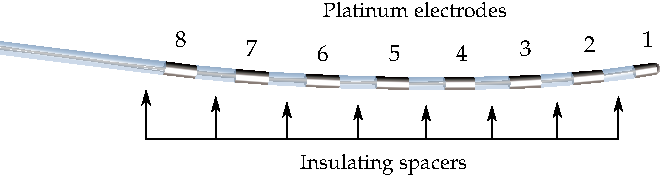
\includegraphics{content/pt2/07-InterfaceModel/graphics/StJudeOctrodeDiagram}
    \caption{\label{fig:StJudeOctrode_Labelled}St. Jude Medical Octrode. An eight electrode array commonly used in spinal stimulation implants.}
  \end{figure}

  \Cref{fig:StJudeOctrode_Labelled} is an illustration of the electrode array and the numbering scheme used to identify each electrode.
  Each electrode on this array is made from platinum and is separated by an insulating spacer.
  The array has eight platinum wires that run through the cable to each of the electrodes.
  This electrode was used through the remainder of this thesis and is the electrode used by Saluda in medical trials of their stimulators.


  \subsection{Inter-electrode resistivity}

  \begin{figure}
    \centering
    \includegraphics{content/pt2/07-InterfaceModel/graphics/electrodeInterface_nonMemristive}
    \caption{\label{fig:pt2-electrodeInterface_nonMemristive}Electrical schematic of the electrode-electrolyte interface}
  \end{figure}

  \subsection{The interface}
    \subsubsection{Constant phase element}
    \subsubsection{Faradaic current}
    \subsubsection{Species depletion}
\section{Methods of Parameter Extraction}
  \subsection{Resistivity and constant phase element}
  \subsection{Faradaic currents}

